\documentclass{beamer}

\usetheme{polimi}




%------------------------------------------------------------------------------
%	REQUIRED PACKAGES AND  CONFIGURATIONS
%------------------------------------------------------------------------------
% PACKAGES FOR TITLES
\usepackage{color}

% PACKAGES FOR LANGUAGE AND FONT
\usepackage[utf8]{inputenc}
\usepackage[english]{babel}
\usepackage[T1]{fontenc} % Font encoding
% PACKAGES FOR IMAGES
\usepackage{graphicx}
\graphicspath{{Images/}} % Path for images' folder
\usepackage{eso-pic} % For the background picture on the title page
\usepackage{subfig} % Numbered and caption subfigures using \subfloat
\usepackage{caption} % Coloured captions
\usepackage{transparent}

% STANDARD MATH PACKAGES
\usepackage{amsmath}
\usepackage{amsthm}
\usepackage{bm}
\usepackage[overload]{empheq}  % For braced-style systems of equations

% PACKAGES FOR TABLES
\usepackage{tabularx}
\usepackage{longtable} % tables that can span several pages
\usepackage{colortbl}

% PACKAGES FOR ALGORITHMS (PSEUDO-CODE)
\usepackage{algorithm}
\usepackage{algorithmic}

% PACKAGES FOR THE APPENDIX
\usepackage{appendix}


% OTHER PACKAGES
\usepackage{amsthm,thmtools,xcolor} % Coloured "Theorem"
\usepackage{comment} % Comment part of code
\usepackage{lipsum} % Insert dummy text
\usepackage{tcolorbox} % Create coloured boxes (e.g. the one for the key-words)
\usepackage{stfloats} % Correct position of the tables
\usepackage{multirow}
\usepackage{multicol}





%-------------------------------------------------------------------------
%	NEW COMMANDS DEFINED
%-------------------------------------------------------------------------
% EXAMPLES OF NEW COMMANDS -> here you see how to define new commands
\newcommand{\bea}{\begin{eqnarray}} % Shortcut for equation arrays
\newcommand{\eea}{\end{eqnarray}}
\newcommand{\e}[1]{\times 10^{#1}}  % Powers of 10 notation
\newcommand{\mathbbm}[1]{\text{\usefont{U}{bbm}{m}{n}#1}} % From mathbbm.sty
\newcommand{\pdev}[2]{\frac{\partial#1}{\partial#2}}
% NB: you can also override some existing commands with the keyword \renewcommand



% \setbeamertemplate{theorem begin}
% {%
%   \par\vskip\medskipamount%
%   \begin{beamercolorbox}[colsep*=.75ex]{block title}
%     \usebeamerfont*{block title}%
%       \inserttheoremname
%       \ifx\inserttheoremaddition\empty\else\ (\inserttheoremaddition)\fi%
%   \end{beamercolorbox}%
%   {\parskip0pt\par}%
%   \ifbeamercolorempty[bg]{block title}
%   {}
%   {\ifbeamercolorempty[bg]{block body}{}{\nointerlineskip\vskip-0.5pt}}%
%   \usebeamerfont{block body}%
%   \vskip-.25ex\vbox{}%
% }
% \setbeamertemplate{theorem end}{}




\newcommand*{\theorembreak}{\(\downarrow\)\usebeamertemplate{theorem end}\framebreak\usebeamertemplate{theorem begin}\rotatebox[origin=c]{180}{$\Lsh$}}





\makeatletter
\newenvironment<>{proofs}[1][\proofname]{%
    \par
    \def\insertproofname{#1\@addpunct{.}}%
    \usebeamertemplate{proof begin}#2}
  {\usebeamertemplate{proof end}}
\newenvironment<>{proofc}{%
  \setbeamertemplate{proof begin}{\begin{block}{}}
    \par
    \usebeamertemplate{proof begin}}
  {\usebeamertemplate{proof end}}
\newenvironment<>{proofe}{%
    \par
    \pushQED{\qed}
    \setbeamertemplate{proof begin}{\begin{block}{}}
    \usebeamertemplate{proof begin}}
  {\popQED\usebeamertemplate{proof end}}






%----------------------------------------------------------------------------
%	ADD YOUR PACKAGES (be careful of package interaction)
%----------------------------------------------------------------------------
\usepackage{amsfonts} 
\usepackage[font=footnotesize,labelfont=bf]{caption}

%----------------------------------------------------------------------------
%	ADD YOUR DEFINITIONS AND COMMANDS (be careful of existing commands)
%----------------------------------------------------------------------------
\usepackage{import}
\usepackage{xifthen}
\usepackage{pdfpages}
\usepackage{transparent}
\usepackage{wrapfig}
\usepackage{dsfont}
\usepackage{tikz}
\usepackage{pgfplots}


\parindent=0pt

\newcommand{\incfig}[1]{%
    \def\svgwidth{\columnwidth}
    \import{./Images/}{#1.pdf_tex}
}
\newcommand{\real}{\mathbb{R}}
\newcommand*{\oldepsilon}{\epsilon}
\renewcommand*{\epsilon}{\varepsilon}
\DeclareMathOperator*{\esssup}{ess\,sup}
\DeclareMathOperator*{\essinf}{ess\,inf}

\newcommand{\oldphi}{\phi}
\renewcommand{\phi}{\varphi}

\newcommand{\oldrho}{\rho}
\renewcommand{\rho}{\varrho}

\numberwithin{equation}{section}
%----------------------------------------------------------------------------
%	CONFIGURATION OF THEOREM ENVIRONMENTS


% \newtheoremstyle{break}
%     {\partopsep}{\topsep}%  
%     {\normalfont}{}
%     {\bfseries}{}%
%     {\newline}{}%
% \theoremstyle{break}
% \newtheorem{theorem}{Theorem}[section]
% \newtheorem{corollary}{Corollary}[section]
% \newtheorem{proposition}{Proposition}[section]
% \newtheorem{remark}{Remark}[section]
% \newtheorem{lemma}{Lemma}[section]
% \newtheorem{notation}{Notation}[section]
% \newtheorem{definition}{Definition}[section]

% \newtheorem{definition}{Definition}[section]

\newtheorem*{remark}{Remark}


\setbeamertemplate{theorems}[numbered]

% %----------------------------------------------------------------------------

% Do not change Configuration_files/config.tex file unless you really know what you are doing.
% This file ends the configuration procedures (e.g. customizing commands, definition of new commands)
% Set the geometric layout of the document
\usepackage{geometry}
\geometry{
  top=3cm,
  left = 2.0cm,
  right = 2.0cm,
  bottom=2cm,
  headheight= 2cm,
  headsep= 0cm,
}
\raggedbottom

% Create color bluePoli (-> manuale grafica coordinata:  https://www.polimi.it/fileadmin/user_upload/il_Politecnico/grafica-coordinata/2015_05_11_46xy_manuale_grafica_coordinata.pdf)
\definecolor{bluePoli}{cmyk}{0.4,0.1,0,0.4}

% Custom theorem environments
\declaretheoremstyle[
  shaded={rulecolor=bluePoli!20, rulewidth=1pt, bgcolor=bluePoli!5},
  headfont=\color{bluePoli}\normalfont\bfseries,
  bodyfont=\color{black}\normalfont,
]{colored}

\captionsetup[figure]{labelfont={color=bluePoli}} % Set colour of the captions
\captionsetup[table]{labelfont={color=bluePoli}} % Set colour of the captions
\captionsetup[algorithm]{labelfont={color=bluePoli}} % Set colour of the captions

\theoremstyle{colored}
\newtheorem{theorem}{Theorem}[section]
\newtheorem{proposition}{Proposition}[section]
\newtheorem{definition}{Definition}[section]
\newtheorem*{remark}{Remark}
\newtheorem{lemma}{Lemma}[section]

% Enhances the features of the standard "table" and "tabular" environments.
\newcommand\T{\rule{0pt}{2.6ex}}
\newcommand\B{\rule[-1.2ex]{0pt}{0pt}}

% Algorithm description
\newcounter{algsubstate}
\renewcommand{\thealgsubstate}{\alph{algsubstate}}
\newenvironment{algsubstates}{
    \setcounter{algsubstate}{0}%
    \renewcommand{\STATE}{%
    \stepcounter{algsubstate}%
    \Statex {\small\thealgsubstate:}\space}
    }{}

% Custom theorem environment
\newcolumntype{L}[1]{>{\raggedright\let\newline\\\arraybackslash\hspace{0pt}}m{#1}}
\newcolumntype{C}[1]{>{\centering\let\newline\\\arraybackslash\hspace{0pt}}m{#1}}
\newcolumntype{R}[1]{>{\raggedleft\let\newline\\\arraybackslash\hspace{0pt}}m{#1}}

% Custom itemize environment
\setlist[itemize,1]{label=$\bullet$}
\setlist[itemize,2]{label=$\circ$}
\setlist[itemize,3]{label=$-$}
\setlist{nosep}

% Set separation of columns
\setlength{\columnsep}{30pt}

% Create command for background pic
\newcommand\BackgroundPic{% Adding background picture
	\put(230,358){
		\parbox[b][\paperheight]{\paperwidth}{%
			\vfill
			\centering
			\transparent{0.2}
			
\includegraphics[width=0.8\paperwidth]{raggiera_polimi.eps}%
			\vfill
}}}

% Set indentation
%\setlength\parindent{0pt}

% Custom title commands
\titleformat{\section}
{\color{bluePoli}\normalfont\Large\bfseries}
{\color{bluePoli}\thesection.}{1em}{}
\titlespacing*{\section}
{0pt}{2ex}{1ex}

\titleformat{\subsection}
{\color{bluePoli}\normalfont\large\bfseries}
{\color{bluePoli}\thesubsection.}{1em}{}
\titlespacing*{\subsection}
{0pt}{2ex}{1ex}

\titleformat{\subsubsection}
{\color{bluePoli}\normalfont\normalsize\bfseries}
{\color{bluePoli}\thesubsubsection.}{1em}{}
\titlespacing*{\subsubsection}
{0pt}{2ex}{1ex}

% Custom headers and footers
\pagestyle{fancy}
\fancyhf{}

\fancyfoot{}
\fancyfoot[C]{\thepage} % page
\renewcommand{\headrulewidth}{0mm} % headrule width
\renewcommand{\footrulewidth}{0mm} % footrule width

\makeatletter
\patchcmd{\headrule}{\hrule}{\color{black}\hrule}{}{} % headrule
\patchcmd{\footrule}{\hrule}{\color{black}\hrule}{}{} % footrule
\makeatother

% -> Create the header
\chead[C]{
\centering
\begin{tcolorbox}[arc=0pt, boxrule=0pt, colback=bluePoli!60, width=\textwidth, colupper=white]
    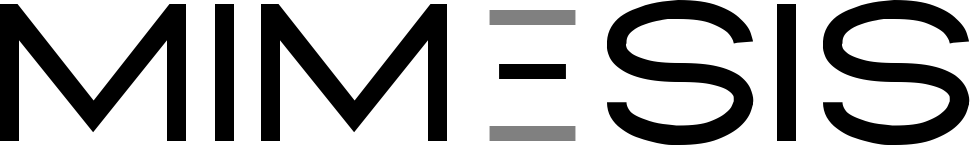
\includegraphics[width=0.2\textwidth]{mimesis.png}
\end{tcolorbox}
}


% Insert here the info that will be displayed into your Title page
% -> title of your work
% -> author name and surname
% -> MSc course
\newcommand\norm[1]{\lVert#1\rVert}





%------------------------------------------------------------------------------
%	TITLE PAGE

%------------------------------------------------------------------------------
\title{The KPP-Fisher equation over simple graphs}
\author{Andrea Bonifacio}

\date{}


\begin{document}

\begin{frame}[plain]
\titlepage
\end{frame}

%------------------------------------------------------------------------------
%	PRESENTATION SLIDES
%------------------------------------------------------------------------------

%------------------------------------------------
\section{Introduction}

% ======================== First Frame ========================

\begin{frame}
    \frametitle{Introduction}
    \begin{itemize}
        \item This report is based on the paper [1], in which the authors study the dynamics of a population in a river network.
        \item The interesting idea proposed in this paper is the study of the population dynamics using a graph-based approach. 
        \item It will be analyzed what changes when the domain is a graph instead of a continuous domain.
    \end{itemize}
\end{frame}

% ======================== Second Frame ========================

\begin{frame}
    \frametitle{Introduction}
    \begin{itemize}
        \item This work will be divided in the following way
        \begin{itemize}
            \item Overview of the results presented in the paper.
            \item Analysis of the theorem on the existence of a solution.
            \item In-depth study of one of the cases presented in the paper.
        \end{itemize}
    \end{itemize}
\end{frame}



%------------------------------------------------

\section{The KPP-Fisher equation}

% ======================== First Frame ========================

\begin{frame}
    \frametitle{Boundary Value Problem}
    The KPP-Fisher equation is a reaction-diffusion equation that models the spread of a population in a given environment. The boundary value problem is given by
    \begin{equation}
        \begin{dcases}
            u_t - D \Delta u = f(\bm{x}, u) & \text{in} \quad Q_T = \Omega \times (0, T), \\
            \partial_{n}u = 0 & \text{on} \quad S_T = \partial \Omega \times (0, T), \\
            u(\bm{x}, 0) = g & \text{in} \quad \Omega,
        \end{dcases}
        \label{eq:fisher-kpp-bvp}
    \end{equation}
    where \(g = g(\bm{x})\) is the initial population density.
\end{frame}

% ======================== Second Frame ========================

\begin{frame}
    \frametitle{Long-time behavior}
    The long-time behavior of the solution of \eqref{eq:fisher-kpp-bvp} is related to the existence of nontrivial steady states \(U = U(\bm{x})\), satisfying:
    \begin{equation}
        \begin{dcases}
            -D \Delta U = f(\bm{x}, U) & \text{in} \quad \Omega, \\
            \partial_{n}U = 0 & \text{on} \quad \partial \Omega.
        \end{dcases}
        \label{eq:fisher-kpp-steady}
    \end{equation}
    This is necessary to understand questions about persistence and extinction of the population.
\end{frame}

% ======================== Third Frame ========================

\begin{frame}
    \frametitle{Supersolutions and subsolutions I}
    In order to understand the behavior of the solution of \eqref{eq:fisher-kpp-bvp}, it is necessary to define supersolutions and subsolutions. 
    \begin{definition}
        A function \(u \in L^2(0, T; V)\) with \(\dot{u} \in L^2(0, T; L^2(\Omega))\), is a weak supersolution (resp. subsolution) of \eqref{eq:fisher-kpp-bvp} if \(u(\bm{x}, 0) \geq g\) (resp. \(u(\bm{x}, 0) \leq g\)) and
        \begin{equation}
            \begin{split}
                \left(\dot{u}(t), v\right)_0 + D \left(\nabla u(t), \nabla v\right)_0 \geq (f(\bm{x}, u(t)), v)_0 \quad \text{(resp } \leq \text{)} \\ \quad \text{for a.e. } t \in (0, T), \forall v \in V, v \geq 0 \text{ a.e. in } \Omega.
            \end{split}
        \end{equation}
    \end{definition}
\end{frame}

% ======================== Fourth Frame ========================

\begin{frame}
    \frametitle{Supersolutions and subsolutions II}
    Another important result related to supersolutions and subsolutions is the following:
    \begin{theorem}
        Let \(\overline{u}\) and \(\underline{u}\) be a bounded weak supersolution and subsolution of \eqref{eq:fisher-kpp-bvp}, respectively. Then, \(\exists!\) weak solution \(u = u_g\) such that
        \begin{equation}
            \underline{u} \leq u_g \leq \overline{u} \quad \text{a.e. in } \quad Q_T.
        \end{equation}
        \label{thm:10.18}
    \end{theorem}
    Thanks to this theorem, it is possible to find a solution that is global in time, meaning that it exists for all \(t > 0\).
\end{frame}

% ======================== Fifth Frame ========================

\begin{frame}
    \frametitle{Supersolutions and subsolutions III}
    \begin{lemma}
        Let \(\phi, \psi \in L^\infty(\Omega) \cap H^1(\Omega)\) be time independent subsolution and supersolution of \eqref{eq:fisher-kpp-bvp}, respectively, and let \(u_\phi, u_\psi\) be the corresponding solutions of the same problem, with initial condition \(u_\phi(0) = \phi\) and \(u_\psi(0) = \psi\). Then
        \begin{enumerate}
            \item \(u_\phi, u_\psi \text{ and } u_g\) exists for all \(t \geq 0\), and 
            \begin{equation}
                \begin{split}
                    \phi(\bm{x}) \leq u_\phi(\bm{x}, t) \leq u_g(\bm{x}, t) \leq u_\psi(\bm{x}, t) \leq \psi(\bm{x}) \\ \quad \text{a.e in } \Omega \times [0, +\infty) \text{ for all }\phi \leq g \leq \psi,
                \end{split}
            \end{equation}
            \item \(u_\phi(\bm{x}, t_2) \geq u_\phi(\bm{x}, t_1)\) a.e. in \(\Omega\), if \(t_2 > t_1\);
            \item \(u_\psi(\bm{x}, t_2) \leq u_\psi(\bm{x}, t_1)\) a.e. in \(\Omega\), if \(t_2 < t_1\).
        \end{enumerate}
        \label{lem:10.21}
    \end{lemma}
\end{frame}

%------------------------------------------------

\section{KPP-Fisher equation over simple graphs}

% ======================== First Frame ========================

\begin{frame}
    \frametitle{The river network}
    Instead of considering a river as a continuous line, here it will be taken into consideration the fact that rivers can divide into smaller rivers and merge into larger rivers. This can be modeled as a graph, where the edges are the rivers and the nodes are the junctions between rivers.
    \tikzset{every picture/.style={line width=0.75pt}} %set default line width to 0.75pt 
\begin{figure}[H]
    \centering
    \scalebox{0.6}{\begin{tikzpicture}[x=0.75pt,y=0.75pt,yscale=-1,xscale=1]
%uncomment if require: \path (0,300); %set diagram left start at 0, and has height of 300

%Straight Lines [id:da06835250339153032] 
\draw    (27.17,139.58) -- (116.96,139.51) ;
\draw [shift={(77.06,139.54)}, rotate = 179.95] [fill={rgb, 255:red, 0; green, 0; blue, 0 }  ][line width=0.08]  [draw opacity=0] (8.93,-4.29) -- (0,0) -- (8.93,4.29) -- cycle    ;
%Shape: Circle [id:dp006568808299004081] 
\draw  [fill={rgb, 255:red, 0; green, 0; blue, 0 }  ,fill opacity=1 ] (114.63,139.51) .. controls (114.63,138.22) and (115.67,137.18) .. (116.96,137.18) .. controls (118.25,137.18) and (119.3,138.22) .. (119.3,139.51) .. controls (119.3,140.8) and (118.25,141.84) .. (116.96,141.84) .. controls (115.67,141.84) and (114.63,140.8) .. (114.63,139.51) -- cycle ;
%Straight Lines [id:da5818375484660003] 
\draw    (456.92,139.33) -- (551.24,139.67) ;
\draw [shift={(509.08,139.52)}, rotate = 180.2] [fill={rgb, 255:red, 0; green, 0; blue, 0 }  ][line width=0.08]  [draw opacity=0] (8.93,-4.29) -- (0,0) -- (8.93,4.29) -- cycle    ;
%Straight Lines [id:da41798667092826824] 
\draw    (120,139.58) -- (210.03,139.58) ;
\draw [shift={(170.01,139.58)}, rotate = 180] [fill={rgb, 255:red, 0; green, 0; blue, 0 }  ][line width=0.08]  [draw opacity=0] (8.93,-4.29) -- (0,0) -- (8.93,4.29) -- cycle    ;
%Shape: Circle [id:dp9495741628591831] 
\draw  [fill={rgb, 255:red, 0; green, 0; blue, 0 }  ,fill opacity=1 ] (548.91,139.67) .. controls (548.91,138.38) and (549.95,137.33) .. (551.24,137.33) .. controls (552.53,137.33) and (553.57,138.38) .. (553.57,139.67) .. controls (553.57,140.96) and (552.53,142) .. (551.24,142) .. controls (549.95,142) and (548.91,140.96) .. (548.91,139.67) -- cycle ;
%Shape: Boxed Line [id:dp3634037576105641] 
\draw    (551.24,139.67) -- (632.76,187.12) ;
\draw [shift={(596.32,165.91)}, rotate = 210.2] [fill={rgb, 255:red, 0; green, 0; blue, 0 }  ][line width=0.08]  [draw opacity=0] (8.93,-4.29) -- (0,0) -- (8.93,4.29) -- cycle    ;
%Shape: Boxed Line [id:dp5855966408278438] 
\draw    (551.24,139.67) -- (633.09,92.79) ;
\draw [shift={(596.5,113.75)}, rotate = 150.2] [fill={rgb, 255:red, 0; green, 0; blue, 0 }  ][line width=0.08]  [draw opacity=0] (8.93,-4.29) -- (0,0) -- (8.93,4.29) -- cycle    ;
%Straight Lines [id:da7091000862619046] 
\draw    (319.92,139.33) -- (414.24,139.67) ;
\draw [shift={(372.08,139.52)}, rotate = 180.2] [fill={rgb, 255:red, 0; green, 0; blue, 0 }  ][line width=0.08]  [draw opacity=0] (8.93,-4.29) -- (0,0) -- (8.93,4.29) -- cycle    ;
%Shape: Boxed Line [id:dp8564221650100632] 
\draw    (240.73,91.88) -- (322.25,139.33) ;
\draw [shift={(285.81,118.12)}, rotate = 210.2] [fill={rgb, 255:red, 0; green, 0; blue, 0 }  ][line width=0.08]  [draw opacity=0] (8.93,-4.29) -- (0,0) -- (8.93,4.29) -- cycle    ;
%Shape: Circle [id:dp5640763569876212] 
\draw  [fill={rgb, 255:red, 0; green, 0; blue, 0 }  ,fill opacity=1 ] (319.92,139.33) .. controls (319.92,138.04) and (320.96,137) .. (322.25,137) .. controls (323.54,137) and (324.58,138.04) .. (324.58,139.33) .. controls (324.58,140.62) and (323.54,141.67) .. (322.25,141.67) .. controls (320.96,141.67) and (319.92,140.62) .. (319.92,139.33) -- cycle ;
%Shape: Boxed Line [id:dp8885765217793992] 
\draw    (240.4,186.21) -- (322.25,139.33) ;
\draw [shift={(285.66,160.28)}, rotate = 150.2] [fill={rgb, 255:red, 0; green, 0; blue, 0 }  ][line width=0.08]  [draw opacity=0] (8.93,-4.29) -- (0,0) -- (8.93,4.29) -- cycle    ;


% Text Node
\draw (35,115.4) node [anchor=north west][inner sep=0.75pt]    {$R_{U}{}{}$};
% Text Node
\draw (465,115.4) node [anchor=north west][inner sep=0.75pt]    {$R_{U}{}{}$};
% Text Node
\draw (169,115.4) node [anchor=north west][inner sep=0.75pt]    {$R_{L}{}{}$};
% Text Node
\draw (378,115.4) node [anchor=north west][inner sep=0.75pt]    {$R_{L}{}{}$};
% Text Node
\draw (592,76.4) node [anchor=north west][inner sep=0.75pt]    {$R_{L_{1}}{}{}$};
% Text Node
\draw (592,173.4) node [anchor=north west][inner sep=0.75pt]    {$R_{L_{2}}{}{}$};
% Text Node
\draw (252,76.4) node [anchor=north west][inner sep=0.75pt]    {$R_{U_{1}}{}{}$};
% Text Node
\draw (254,177.4) node [anchor=north west][inner sep=0.75pt]    {$R_{U_{2}}{}{}$};
% Text Node
\draw (28,200) node [anchor=north west][inner sep=0.75pt]   [align=left] {a)};
% Text Node
\draw (240,200) node [anchor=north west][inner sep=0.75pt]   [align=left] {b)};
% Text Node
\draw (458,200) node [anchor=north west][inner sep=0.75pt]   [align=left] {c)};


\end{tikzpicture}}
    \caption{Graph representation of the river. a) The river is split in an upper branch \(R_U\) and a lower branch \(R_L\). b) The upper branch is split in two branches \(R_{U_1}\) and \(R_{U_2}\). c) The lower branch is split in two branches \(R_{L_1}\) and \(R_{L_2}\).}
    \label{fig:river-graph}
\end{figure}
\end{frame}

% ======================== Second Frame ========================

\begin{frame}
    \frametitle{Steady states}
    With the graph based approach, infinitely many steady states can exist. However, only one of them can be a global attractor. And these global attractors can be summed up in three types:
    \begin{enumerate}
        \item \textbf{washing out:} the population density goes to zero in all the branches;
        \item \textbf{persistence at carrying capacity:} the population survives in all the branches;
        \item \textbf{persistence below carrying capacity:} the population density goes to a value below the carrying capacity in some branches.
    \end{enumerate}
\end{frame}

% ======================== Third Frame ========================

\begin{frame}
    \frametitle{One upper branch and one lower branch I}
    Consider the case where the river is split in an upper branch \(R_U\) and a lower branch \(R_L\). The system of equations is given by
    \begin{equation}
        \begin{dcases}
            \partial_t w_L - \partial_{xx}w_L + \beta_L \partial_x w_L = w_L(1 - w_L) &  x \in \real_L, t > 0, \\
            \partial_t w_U - \partial_{xx}w_U + \beta_U \partial_x w_U = w_U(1 - w_U) & x \in \real_U, t > 0, \\
            w_L(0, t) = w_U(0, t) &  t > 0, \\
            a_L \partial_x w_L(0, t) = a_U \partial_x w_U(0, t) &  t > 0, \\
            w_L(x, 0) = w_{0}(x) &  x \in \real_L, \\
            w_U(x, 0) = w_{0}(x) &  x \in \real_U.
        \end{dcases}
        \label{eq:1.6}
    \end{equation}
\end{frame}

% ======================== Fourth Frame ========================

\begin{frame}
    \frametitle{One upper branch and one lower branch II}
    In Equation \eqref{eq:1.6} the parameters \(\beta_L\) and \(\beta_U\) are the diffusion coefficients in the lower and upper branches, respectively. The parameters \(a_L\) and \(a_U\) are the coefficients of the advection terms in the lower and upper branches, respectively. The initial condition is the same for both branches and is given by \(w_0(x) \in C_{comp}(\real)\), where \(C_{comp}(\real)\) is the set of continuous functions with compact support in \(\real\).

    The compactness of the support of the initial condition is crucial to determine the long-time behavior of the solution. In fact, the steady state chosen as the global attractor is the one that decays to zero faster at infinity.
\end{frame}

% ======================== Fifth Frame ========================

\begin{frame}
    \frametitle{One upper branch and one lower branch III}
    The long-time behavior of the solution of \eqref{eq:1.6} is related to the solutions of the stationary problem
    \begin{equation}
        \begin{dcases}
            - \ddot{\phi}_L + \beta_L \dot{\phi}_L = \phi_L(1 - \phi_L), & 0 < \phi_L < 1, x \in \real_L, \\
            - \ddot{\phi}_U + \beta_U \dot{\phi}_U = \phi_U(1 - \phi_U), & 0 < \phi_U < 1, x \in \real_U, \\
            \phi_L(0) = \phi_U(0) = \alpha \in [0, 1], \\
            a_L \dot{\phi}_L(0) = a_U \dot{\phi}_U(0).
        \end{dcases}
        \label{eq:1.8}
    \end{equation}
\end{frame}

% ======================== Sixth Frame ========================

\begin{frame}[allowframebreaks]
    \frametitle{Behaviour of solutions}
    The following theorems shed some light on the behavior of the solutions of \eqref{eq:1.6} and their long-time dynamics.
    \begin{theorem}
        Since the assumption is that \(D_L = D_U = 1\), the maximum speed of the population invasion is \(c_* = 2\). 
        
        (i) If \(0 < \beta_U < 2\), then \eqref{eq:1.8} has no solution for \(\alpha \in (0, 1)\). 


        (ii) If \(\beta_L, \beta_U \geq 2\), then for every \(\alpha \in (0, 1)\) \eqref{eq:1.8} has a unique solution.


        (iii) If \(\beta_U \geq 2 > \beta_L > 0\), then there exists \(\alpha_0 \in (0, 1)\) such that \eqref{eq:1.8} has a unique solution for each \(\alpha \in [\alpha_0, 1)\), and no solution for \(\alpha \in (0, \alpha_0)\).

        \theorembreak
        (iv)  Whenever \eqref{eq:1.8} has a solution \((\phi_L, \phi_U)\), it is true that 
            \[
                \dot{\phi}_L > 0, \quad \dot{\phi}_U > 0, \quad \phi_L(\infty) = 1, \quad \phi_U(-\infty) = 0.
            \]
            Moreover, in case (ii) and (iii) with \(\alpha \in [\alpha_0, 1)\), as \(x \to -\infty\), there exists some \(c = c(\alpha) > 0\) such that
            \begin{equation}
                \phi_U(x) = \begin{cases}
                    (c + o(1))e^{\frac{1}{2}(\beta_U - \sqrt{\beta_U^2 - 4})x} & \text{if } \beta_U > 2, \\
                    (c + o(1))\lvert x\rvert e^{x} & \text{if } \beta_U = 2, \\
                \end{cases} 
                \label{eq:1.9}
            \end{equation}
        \theorembreak
            while in case (iii) with \(\alpha = \alpha_0\), as \(x \to -\infty\), there exists some \(c > 0\) such that
            \begin{equation}
                \phi_U(x) = (c + o(1))e^{\frac{1}{2}(\beta_U - \sqrt{\beta_U^2 - 4})x}.
                \label{eq:1.10}
            \end{equation}
        \label{thm:1.1}
    \end{theorem}
\end{frame}

% ======================== Seventh Frame ========================

\begin{frame}[allowframebreaks]
    \frametitle{Long-time dynamics}
    \begin{theorem}
        Assuming that \(w_0 \in C_{comp}(\real)\) is nonnegative and nontrivial, let \((w_L, w_U)\) be the solution of \eqref{eq:1.6}. Then the following holds:

            (i) If \(0 < \beta_U < 2\), then \((w_L(\cdot, t), w_U(\cdot, t)) \to (1, 1)\) locally uniformly as \(t \to +\infty\).

            (ii) If \(\beta_U, \beta_L \geq 2\), then \((w_L(\cdot, t), w_U(\cdot, t)) \to (0, 0)\) locally uniformly as \(t \to +\infty\). Also, \(\norm{w_L(\cdot, t)}_{L^\infty(\real_L)} \to 1\) and \(\norm{w_U(\cdot, t)}_{L^\infty(\real_U)} \to 0\) as \(t \to +\infty\).
            \theorembreak
            (iii) If \(\beta_U \geq 2 > \beta_L > 0\), then \((w_L(\cdot, t), w_U(\cdot, t)) \to (\phi_L(\cdot; \alpha_0), \phi_U(\cdot; \alpha_0))\)\footnote{\((\phi_L(\cdot; \alpha_0), \phi_U(\cdot; \alpha_0))\) is the unique solution of \eqref{eq:1.8} with \(\alpha = \alpha_0\).} locally uniformly as \(t \to +\infty\).
        \label{thm:1.2}
    \end{theorem}
\end{frame}

% ======================== Eighth Frame ========================

\begin{frame}
    \frametitle{Long-time dynamics III}
    In case (ii) of Theorem \ref{thm:1.2}, the population density goes to zero locally in all the branches, because the river's flow is too strong for the population to survive. However, the \(L^\infty\) norm of the population density in the lower branch goes to \(1\), meaning that the population is not out of the network.

    In case (i) and (ii) it is clear that it's far more important the advection coefficient of the upper branch.

    The last case shows that the steady state solution is increasing in both branches, and its limit at \(x \to -\infty\) is 0, while at \(x \to +\infty\) is 1. This is the selected steady state because it decays to zero faster at infinity.
\end{frame}

%------------------------------------------------

\end{document}